\documentclass{standalone}
\usepackage{tikz}
\usepackage{xcolor}

\usetikzlibrary{decorations.pathmorphing}
\usetikzlibrary{shapes}
\usetikzlibrary{shapes.geometric}

\tikzset{
	magnetic/.style={
		fill,
		shape border rotate=0,
		isosceles triangle,
		isosceles triangle apex angle=60,
		%fill=red,
		node distance=1,
		minimum height=.1
	}
}

\tikzset{
	othermagnetic/.style={
		fill,
		shape border rotate=90,
		isosceles triangle,
		isosceles triangle apex angle=60,
		%fill=red,
		node distance=1,
		minimum height=.1
	}
}


\begin{document}
	
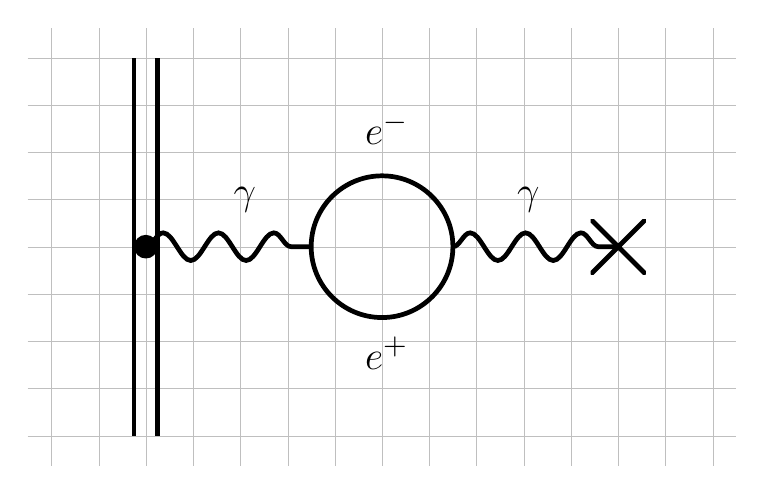
\begin{tikzpicture}[ thick,scale=3,cross/.style={path picture={ 
			\draw[black]
			(path picture bounding box.south east) -- (path picture bounding box.north west) (path picture bounding box.south west) -- (path picture bounding box.north east);
	}}]
	
	% (VP_ml-B)
	\draw[gray!50,line width=0.01mm,step=0.2] (-0.5,0.073) grid (2.5, 1.927);
\draw[line width =0.6mm] (-0.05, 0.2) -- (-0.05, 1.8);
\draw[line width=0.6mm] (+0.05, 0.2) -- ( 0.05, 1.8);
\fill (0,1) circle (0.05);
\draw[decorate,decoration={snake,amplitude=5,segment length=20},line width=0.6mm] (0,1)  -- (0.7,1);
%\fill (1.5,2.5) circle (0.1);
	\draw[line width=0.6mm] (1,1) circle (0.3);
	%\fill (3.5,2.5) circle (0.1);
	\draw[decorate,decoration={snake,amplitude=5,segment length=20},line width=0.6mm] (1.3,1)  -- (2,1);
	%\draw[inner sep=2] (4,2.5) node [magnetic]{};
\node [cross,line width=0.6 mm,minimum size=7mm] at (2,1){};
	\node at (0.4,1.2) {\fontsize{15pt}{0} $\gamma$};
	\node at (1.6,1.2) {\fontsize{15pt}{0} $\gamma$};
	\node at (1,1.5) {\fontsize{15pt}{0} $e^-$};
	\node at (1,0.55) {\fontsize{15pt}{0} $e^+$};

\end{tikzpicture}

\end{document}

$ \Delta E_{NP} = \alpha \sum\limits_{\omega_L,L} \sum\limits_n \frac{\langle a |\delta V_{\rm NP}(\omega_L) | n \rangle }{\epsilon_a - \epsilon_n - {\rm sign}(\epsilon_n)\omega_L}$

